% PREAMBLE
\documentclass[11pt]{amsart}
\usepackage[T1]{fontenc}
\usepackage{lmodern}
\usepackage{microtype}
\usepackage{amsmath,amssymb}
\usepackage{mathtools}
\usepackage{graphicx}
\usepackage{booktabs}
\usepackage{tikz}
\usepackage[colorlinks=true,linkcolor=blue!45!black,citecolor=blue!45!black,urlcolor=blue!45!black]{hyperref}
\usepackage[capitalize]{cleveref}

\newtheorem{theorem}{Theorem}[section]
\newtheorem{proposition}[theorem]{Proposition}
\newtheorem{lemma}[theorem]{Lemma}
\newtheorem{corollary}[theorem]{Corollary}
\newtheorem{conjecture}[theorem]{Conjecture}
\theoremstyle{definition}
\newtheorem{definition}[theorem]{Definition}
\newtheorem{fact}[theorem]{Fact}
\theoremstyle{remark}
\newtheorem{remark}[theorem]{Remark}

\title[The Walsh Spectrometer]{The Walsh Spectrometer: Exact Diagonal-Slice Ink for Every Three-Dimensional Parity Design}
\author{Carlo Mitchener}
\address{MrlyProd, Inc.}
\email{carlo.mitchener@gmail.com}
\date{First published 2026-08-23, revised 2026-09-03}

% PAPER
\begin{document}

\begin{abstract}
Colour the cells of a cube by a rule that looks only at whether each coordinate lies in an even or an odd block, then cut the cube with a slanted plane and ask what fraction of the cut is coloured. There are exactly $256$ such rules, and this paper answers the question for all of them at once, exactly and with no error term. The answer is an exact quasipolynomial in one over the size parameter, of period four in that parameter, and its six coefficients are not fitted numbers: they are the sums of the rule's Walsh--Fourier coefficients, level by level, with complementary levels paired across orders.
\end{abstract}

% TITLE PAGE
\makeatletter
\global\let\titledate\@date
\global\let\paperabstract\@setabstracta
\global\let\@date\@empty
\global\let\@setabstract\relax
\makeatother

\maketitle

\begin{center}
\normalfont\footnotesize\titledate
\end{center}

\vspace*{\stretch{1}}

\begin{center}

\includegraphics[width=0.5\textwidth]{figures/avatar.png}
\end{center}

\vspace*{\stretch{1.25}}

\newpage

\paperabstract

% BODY
\section{Introduction}
\label{sec:intro}

Take a big cube of graph paper, $4n$ cells on a side. Chop each axis into blocks of four, so the cube is an $n \times n \times n$ arrangement of $4 \times 4 \times 4$ blocks. Every cell now carries three bits: is its $x$-block even or odd, its $y$-block, its $z$-block. That triple of bits is the cell's \emph{macro parity}, and it takes eight values, the corners of a cube.

A \emph{design} is a decision about those eight corners: for each one, ink or paper. There are $2^8 = 256$ designs, and each is a way of painting the cube in a coarse checkerboard.

\begin{figure}[!ht]
\centering
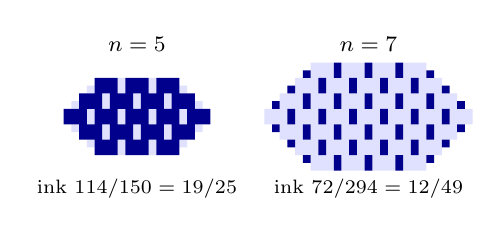
\begin{tikzpicture}[scale=0.098]
\begin{scope}[shift={(0,4)}]
\fill[blue!12] (-2,5) rectangle ++(1,1) (2,5) rectangle ++(1,1) (-6,6) rectangle ++(1,1) (-2,6) rectangle ++(1,1) (2,6) rectangle ++(1,1) (6,6) rectangle ++(1,1) (-4,7) rectangle ++(1,1) (0,7) rectangle ++(1,1) (4,7) rectangle ++(1,1) (-8,8) rectangle ++(1,1) (-4,8) rectangle ++(1,1) (0,8) rectangle ++(1,1) (4,8) rectangle ++(1,1) (8,8) rectangle ++(1,1) (-6,9) rectangle ++(1,1) (-2,9) rectangle ++(1,1) (2,9) rectangle ++(1,1) (6,9) rectangle ++(1,1) (-6,10) rectangle ++(1,1) (-2,10) rectangle ++(1,1) (2,10) rectangle ++(1,1) (6,10) rectangle ++(1,1) (-8,11) rectangle ++(1,1) (-4,11) rectangle ++(1,1) (0,11) rectangle ++(1,1) (4,11) rectangle ++(1,1) (8,11) rectangle ++(1,1) (-4,12) rectangle ++(1,1) (0,12) rectangle ++(1,1) (4,12) rectangle ++(1,1) (-6,13) rectangle ++(1,1) (-2,13) rectangle ++(1,1) (2,13) rectangle ++(1,1) (6,13) rectangle ++(1,1) (-2,14) rectangle ++(1,1) (2,14) rectangle ++(1,1);
\fill[blue!55!black] (-5,5) rectangle ++(1,1) (-4,5) rectangle ++(1,1) (-3,5) rectangle ++(1,1) (-1,5) rectangle ++(1,1) (0,5) rectangle ++(1,1) (1,5) rectangle ++(1,1) (3,5) rectangle ++(1,1) (4,5) rectangle ++(1,1) (5,5) rectangle ++(1,1) (-5,6) rectangle ++(1,1) (-4,6) rectangle ++(1,1) (-3,6) rectangle ++(1,1) (-1,6) rectangle ++(1,1) (0,6) rectangle ++(1,1) (1,6) rectangle ++(1,1) (3,6) rectangle ++(1,1) (4,6) rectangle ++(1,1) (5,6) rectangle ++(1,1) (-7,7) rectangle ++(1,1) (-6,7) rectangle ++(1,1) (-5,7) rectangle ++(1,1) (-3,7) rectangle ++(1,1) (-2,7) rectangle ++(1,1) (-1,7) rectangle ++(1,1) (1,7) rectangle ++(1,1) (2,7) rectangle ++(1,1) (3,7) rectangle ++(1,1) (5,7) rectangle ++(1,1) (6,7) rectangle ++(1,1) (7,7) rectangle ++(1,1) (-7,8) rectangle ++(1,1) (-6,8) rectangle ++(1,1) (-5,8) rectangle ++(1,1) (-3,8) rectangle ++(1,1) (-2,8) rectangle ++(1,1) (-1,8) rectangle ++(1,1) (1,8) rectangle ++(1,1) (2,8) rectangle ++(1,1) (3,8) rectangle ++(1,1) (5,8) rectangle ++(1,1) (6,8) rectangle ++(1,1) (7,8) rectangle ++(1,1) (-9,9) rectangle ++(1,1) (-8,9) rectangle ++(1,1) (-7,9) rectangle ++(1,1) (-5,9) rectangle ++(1,1) (-4,9) rectangle ++(1,1) (-3,9) rectangle ++(1,1) (-1,9) rectangle ++(1,1) (0,9) rectangle ++(1,1) (1,9) rectangle ++(1,1) (3,9) rectangle ++(1,1) (4,9) rectangle ++(1,1) (5,9) rectangle ++(1,1) (7,9) rectangle ++(1,1) (8,9) rectangle ++(1,1) (9,9) rectangle ++(1,1) (-9,10) rectangle ++(1,1) (-8,10) rectangle ++(1,1) (-7,10) rectangle ++(1,1) (-5,10) rectangle ++(1,1) (-4,10) rectangle ++(1,1) (-3,10) rectangle ++(1,1) (-1,10) rectangle ++(1,1) (0,10) rectangle ++(1,1) (1,10) rectangle ++(1,1) (3,10) rectangle ++(1,1) (4,10) rectangle ++(1,1) (5,10) rectangle ++(1,1) (7,10) rectangle ++(1,1) (8,10) rectangle ++(1,1) (9,10) rectangle ++(1,1) (-7,11) rectangle ++(1,1) (-6,11) rectangle ++(1,1) (-5,11) rectangle ++(1,1) (-3,11) rectangle ++(1,1) (-2,11) rectangle ++(1,1) (-1,11) rectangle ++(1,1) (1,11) rectangle ++(1,1) (2,11) rectangle ++(1,1) (3,11) rectangle ++(1,1) (5,11) rectangle ++(1,1) (6,11) rectangle ++(1,1) (7,11) rectangle ++(1,1) (-7,12) rectangle ++(1,1) (-6,12) rectangle ++(1,1) (-5,12) rectangle ++(1,1) (-3,12) rectangle ++(1,1) (-2,12) rectangle ++(1,1) (-1,12) rectangle ++(1,1) (1,12) rectangle ++(1,1) (2,12) rectangle ++(1,1) (3,12) rectangle ++(1,1) (5,12) rectangle ++(1,1) (6,12) rectangle ++(1,1) (7,12) rectangle ++(1,1) (-5,13) rectangle ++(1,1) (-4,13) rectangle ++(1,1) (-3,13) rectangle ++(1,1) (-1,13) rectangle ++(1,1) (0,13) rectangle ++(1,1) (1,13) rectangle ++(1,1) (3,13) rectangle ++(1,1) (4,13) rectangle ++(1,1) (5,13) rectangle ++(1,1) (-5,14) rectangle ++(1,1) (-4,14) rectangle ++(1,1) (-3,14) rectangle ++(1,1) (-1,14) rectangle ++(1,1) (0,14) rectangle ++(1,1) (1,14) rectangle ++(1,1) (3,14) rectangle ++(1,1) (4,14) rectangle ++(1,1) (5,14) rectangle ++(1,1);
\node[font=\footnotesize] at (0.5,19.4) {$n = 5$};
\node[font=\scriptsize] at (0.5,0.6) {ink $114/150 = 19/25$};
\end{scope}
\begin{scope}[shift={(30,0)}]
\fill[blue!12] (-7,7) rectangle ++(1,1) (-6,7) rectangle ++(1,1) (-5,7) rectangle ++(1,1) (-3,7) rectangle ++(1,1) (-2,7) rectangle ++(1,1) (-1,7) rectangle ++(1,1) (1,7) rectangle ++(1,1) (2,7) rectangle ++(1,1) (3,7) rectangle ++(1,1) (5,7) rectangle ++(1,1) (6,7) rectangle ++(1,1) (7,7) rectangle ++(1,1) (-7,8) rectangle ++(1,1) (-6,8) rectangle ++(1,1) (-5,8) rectangle ++(1,1) (-3,8) rectangle ++(1,1) (-2,8) rectangle ++(1,1) (-1,8) rectangle ++(1,1) (1,8) rectangle ++(1,1) (2,8) rectangle ++(1,1) (3,8) rectangle ++(1,1) (5,8) rectangle ++(1,1) (6,8) rectangle ++(1,1) (7,8) rectangle ++(1,1) (-9,9) rectangle ++(1,1) (-8,9) rectangle ++(1,1) (-7,9) rectangle ++(1,1) (-5,9) rectangle ++(1,1) (-4,9) rectangle ++(1,1) (-3,9) rectangle ++(1,1) (-1,9) rectangle ++(1,1) (0,9) rectangle ++(1,1) (1,9) rectangle ++(1,1) (3,9) rectangle ++(1,1) (4,9) rectangle ++(1,1) (5,9) rectangle ++(1,1) (7,9) rectangle ++(1,1) (8,9) rectangle ++(1,1) (9,9) rectangle ++(1,1) (-9,10) rectangle ++(1,1) (-8,10) rectangle ++(1,1) (-7,10) rectangle ++(1,1) (-5,10) rectangle ++(1,1) (-4,10) rectangle ++(1,1) (-3,10) rectangle ++(1,1) (-1,10) rectangle ++(1,1) (0,10) rectangle ++(1,1) (1,10) rectangle ++(1,1) (3,10) rectangle ++(1,1) (4,10) rectangle ++(1,1) (5,10) rectangle ++(1,1) (7,10) rectangle ++(1,1) (8,10) rectangle ++(1,1) (9,10) rectangle ++(1,1) (-11,11) rectangle ++(1,1) (-10,11) rectangle ++(1,1) (-9,11) rectangle ++(1,1) (-7,11) rectangle ++(1,1) (-6,11) rectangle ++(1,1) (-5,11) rectangle ++(1,1) (-3,11) rectangle ++(1,1) (-2,11) rectangle ++(1,1) (-1,11) rectangle ++(1,1) (1,11) rectangle ++(1,1) (2,11) rectangle ++(1,1) (3,11) rectangle ++(1,1) (5,11) rectangle ++(1,1) (6,11) rectangle ++(1,1) (7,11) rectangle ++(1,1) (9,11) rectangle ++(1,1) (10,11) rectangle ++(1,1) (11,11) rectangle ++(1,1) (-11,12) rectangle ++(1,1) (-10,12) rectangle ++(1,1) (-9,12) rectangle ++(1,1) (-7,12) rectangle ++(1,1) (-6,12) rectangle ++(1,1) (-5,12) rectangle ++(1,1) (-3,12) rectangle ++(1,1) (-2,12) rectangle ++(1,1) (-1,12) rectangle ++(1,1) (1,12) rectangle ++(1,1) (2,12) rectangle ++(1,1) (3,12) rectangle ++(1,1) (5,12) rectangle ++(1,1) (6,12) rectangle ++(1,1) (7,12) rectangle ++(1,1) (9,12) rectangle ++(1,1) (10,12) rectangle ++(1,1) (11,12) rectangle ++(1,1) (-13,13) rectangle ++(1,1) (-12,13) rectangle ++(1,1) (-11,13) rectangle ++(1,1) (-9,13) rectangle ++(1,1) (-8,13) rectangle ++(1,1) (-7,13) rectangle ++(1,1) (-5,13) rectangle ++(1,1) (-4,13) rectangle ++(1,1) (-3,13) rectangle ++(1,1) (-1,13) rectangle ++(1,1) (0,13) rectangle ++(1,1) (1,13) rectangle ++(1,1) (3,13) rectangle ++(1,1) (4,13) rectangle ++(1,1) (5,13) rectangle ++(1,1) (7,13) rectangle ++(1,1) (8,13) rectangle ++(1,1) (9,13) rectangle ++(1,1) (11,13) rectangle ++(1,1) (12,13) rectangle ++(1,1) (13,13) rectangle ++(1,1) (-13,14) rectangle ++(1,1) (-12,14) rectangle ++(1,1) (-11,14) rectangle ++(1,1) (-9,14) rectangle ++(1,1) (-8,14) rectangle ++(1,1) (-7,14) rectangle ++(1,1) (-5,14) rectangle ++(1,1) (-4,14) rectangle ++(1,1) (-3,14) rectangle ++(1,1) (-1,14) rectangle ++(1,1) (0,14) rectangle ++(1,1) (1,14) rectangle ++(1,1) (3,14) rectangle ++(1,1) (4,14) rectangle ++(1,1) (5,14) rectangle ++(1,1) (7,14) rectangle ++(1,1) (8,14) rectangle ++(1,1) (9,14) rectangle ++(1,1) (11,14) rectangle ++(1,1) (12,14) rectangle ++(1,1) (13,14) rectangle ++(1,1) (-11,15) rectangle ++(1,1) (-10,15) rectangle ++(1,1) (-9,15) rectangle ++(1,1) (-7,15) rectangle ++(1,1) (-6,15) rectangle ++(1,1) (-5,15) rectangle ++(1,1) (-3,15) rectangle ++(1,1) (-2,15) rectangle ++(1,1) (-1,15) rectangle ++(1,1) (1,15) rectangle ++(1,1) (2,15) rectangle ++(1,1) (3,15) rectangle ++(1,1) (5,15) rectangle ++(1,1) (6,15) rectangle ++(1,1) (7,15) rectangle ++(1,1) (9,15) rectangle ++(1,1) (10,15) rectangle ++(1,1) (11,15) rectangle ++(1,1) (-11,16) rectangle ++(1,1) (-10,16) rectangle ++(1,1) (-9,16) rectangle ++(1,1) (-7,16) rectangle ++(1,1) (-6,16) rectangle ++(1,1) (-5,16) rectangle ++(1,1) (-3,16) rectangle ++(1,1) (-2,16) rectangle ++(1,1) (-1,16) rectangle ++(1,1) (1,16) rectangle ++(1,1) (2,16) rectangle ++(1,1) (3,16) rectangle ++(1,1) (5,16) rectangle ++(1,1) (6,16) rectangle ++(1,1) (7,16) rectangle ++(1,1) (9,16) rectangle ++(1,1) (10,16) rectangle ++(1,1) (11,16) rectangle ++(1,1) (-9,17) rectangle ++(1,1) (-8,17) rectangle ++(1,1) (-7,17) rectangle ++(1,1) (-5,17) rectangle ++(1,1) (-4,17) rectangle ++(1,1) (-3,17) rectangle ++(1,1) (-1,17) rectangle ++(1,1) (0,17) rectangle ++(1,1) (1,17) rectangle ++(1,1) (3,17) rectangle ++(1,1) (4,17) rectangle ++(1,1) (5,17) rectangle ++(1,1) (7,17) rectangle ++(1,1) (8,17) rectangle ++(1,1) (9,17) rectangle ++(1,1) (-9,18) rectangle ++(1,1) (-8,18) rectangle ++(1,1) (-7,18) rectangle ++(1,1) (-5,18) rectangle ++(1,1) (-4,18) rectangle ++(1,1) (-3,18) rectangle ++(1,1) (-1,18) rectangle ++(1,1) (0,18) rectangle ++(1,1) (1,18) rectangle ++(1,1) (3,18) rectangle ++(1,1) (4,18) rectangle ++(1,1) (5,18) rectangle ++(1,1) (7,18) rectangle ++(1,1) (8,18) rectangle ++(1,1) (9,18) rectangle ++(1,1) (-7,19) rectangle ++(1,1) (-6,19) rectangle ++(1,1) (-5,19) rectangle ++(1,1) (-3,19) rectangle ++(1,1) (-2,19) rectangle ++(1,1) (-1,19) rectangle ++(1,1) (1,19) rectangle ++(1,1) (2,19) rectangle ++(1,1) (3,19) rectangle ++(1,1) (5,19) rectangle ++(1,1) (6,19) rectangle ++(1,1) (7,19) rectangle ++(1,1) (-7,20) rectangle ++(1,1) (-6,20) rectangle ++(1,1) (-5,20) rectangle ++(1,1) (-3,20) rectangle ++(1,1) (-2,20) rectangle ++(1,1) (-1,20) rectangle ++(1,1) (1,20) rectangle ++(1,1) (2,20) rectangle ++(1,1) (3,20) rectangle ++(1,1) (5,20) rectangle ++(1,1) (6,20) rectangle ++(1,1) (7,20) rectangle ++(1,1);
\fill[blue!55!black] (-4,7) rectangle ++(1,1) (0,7) rectangle ++(1,1) (4,7) rectangle ++(1,1) (-8,8) rectangle ++(1,1) (-4,8) rectangle ++(1,1) (0,8) rectangle ++(1,1) (4,8) rectangle ++(1,1) (8,8) rectangle ++(1,1) (-6,9) rectangle ++(1,1) (-2,9) rectangle ++(1,1) (2,9) rectangle ++(1,1) (6,9) rectangle ++(1,1) (-10,10) rectangle ++(1,1) (-6,10) rectangle ++(1,1) (-2,10) rectangle ++(1,1) (2,10) rectangle ++(1,1) (6,10) rectangle ++(1,1) (10,10) rectangle ++(1,1) (-8,11) rectangle ++(1,1) (-4,11) rectangle ++(1,1) (0,11) rectangle ++(1,1) (4,11) rectangle ++(1,1) (8,11) rectangle ++(1,1) (-12,12) rectangle ++(1,1) (-8,12) rectangle ++(1,1) (-4,12) rectangle ++(1,1) (0,12) rectangle ++(1,1) (4,12) rectangle ++(1,1) (8,12) rectangle ++(1,1) (12,12) rectangle ++(1,1) (-10,13) rectangle ++(1,1) (-6,13) rectangle ++(1,1) (-2,13) rectangle ++(1,1) (2,13) rectangle ++(1,1) (6,13) rectangle ++(1,1) (10,13) rectangle ++(1,1) (-10,14) rectangle ++(1,1) (-6,14) rectangle ++(1,1) (-2,14) rectangle ++(1,1) (2,14) rectangle ++(1,1) (6,14) rectangle ++(1,1) (10,14) rectangle ++(1,1) (-12,15) rectangle ++(1,1) (-8,15) rectangle ++(1,1) (-4,15) rectangle ++(1,1) (0,15) rectangle ++(1,1) (4,15) rectangle ++(1,1) (8,15) rectangle ++(1,1) (12,15) rectangle ++(1,1) (-8,16) rectangle ++(1,1) (-4,16) rectangle ++(1,1) (0,16) rectangle ++(1,1) (4,16) rectangle ++(1,1) (8,16) rectangle ++(1,1) (-10,17) rectangle ++(1,1) (-6,17) rectangle ++(1,1) (-2,17) rectangle ++(1,1) (2,17) rectangle ++(1,1) (6,17) rectangle ++(1,1) (10,17) rectangle ++(1,1) (-6,18) rectangle ++(1,1) (-2,18) rectangle ++(1,1) (2,18) rectangle ++(1,1) (6,18) rectangle ++(1,1) (-8,19) rectangle ++(1,1) (-4,19) rectangle ++(1,1) (0,19) rectangle ++(1,1) (4,19) rectangle ++(1,1) (8,19) rectangle ++(1,1) (-4,20) rectangle ++(1,1) (0,20) rectangle ++(1,1) (4,20) rectangle ++(1,1);
\node[font=\footnotesize] at (0.5,23.4) {$n = 7$};
\node[font=\scriptsize] at (0.5,4.6) {ink $72/294 = 12/49$};
\end{scope}
\end{tikzpicture}
\caption{Code $105$, which inks a cell when its macro parity has even weight, at two consecutive odd sizes. Its ink is $\tfrac12 - \tfrac14 s - \tfrac{s}{4n^2}$ with $s = -1$ for $n \equiv 1$ and $s=+1$ for $n \equiv 3 \pmod 4$: the picture flips forever, and the amplitude $\tfrac14$ is minus half its top Walsh coefficient.}
\label{fig:blink}
\end{figure}

Now cut. Take the slanted plane $x+y+z = 6n-2$ and keep only the cells on it with $z$ even. The cut is a hexagon of exactly $6n^2$ cells. Ink it with the design and ask the only question a picture can answer: what fraction of the hexagon is inked? Call it $\mathrm{ink}_D(n)$.



The surprise is that this fraction is never messy and never needs a fit. It is an exact rational function of $n$ with a two-step wobble, and its coefficients are the design's spectrum.


Here is the whole story in one line. Let $F(S)$ be the Walsh--Fourier coefficients of the design's indicator function on $\{0,1\}^3$, and let $\Sigma_j$ be the sum of the $\binom{3}{j}$ coefficients at level $j$. Then for every odd $n$,
\[
\mathrm{ink}_D(n) = \Sigma_0 - \tfrac12 \Sigma_3\, s
 + \frac{\tfrac23 \Sigma_1 - \tfrac13 \Sigma_2\, s}{n}
 + \frac{\tfrac23 \Sigma_2 - \bigl(\tfrac13 \Sigma_1 + \tfrac12 \Sigma_3\bigr) s}{n^2},
\]
where $s = (-1)^{(3n-1)/2}$. Read it as an instrument. The steady background is the mean Walsh coefficient. The two-step blink is minus half the top Walsh coefficient and nothing else. The $1/n$ and $1/n^2$ orders carry the two middle levels, and the alternating part reads the level the steady part does not, $j$ against $3-j$, with the top level riding along once more in the last term. That is why we call the layer stack a spectrometer. Point it at a design and it prints the design's spectrum.

\subsection*{What is new and what is not}

That the counts here are quasipolynomial in $n$ is not new and should not be sold as new. The point set is the lattice-point set of a rational polytope, a hexagonal cross-section of a cube, refined by congruence conditions on the coordinates. Ehrhart's theorem and its extension to lattice points in dilates under congruence side conditions \cite{ehrhart,beckrobins} already guarantee a quasipolynomial of degree $2$ whose period divides $4$, and Barvinok's algorithm \cite{barvinok}, as implemented in LattE \cite{latte}, will produce every constituent mechanically. Anyone who expected these counts to be quasipolynomial was right.

Three things here are not mechanical. First, the closed forms are written down, in a shape short enough to use: eight quadratics with denominator $8$. Second, the counts depend only on the \emph{weight} of the macro-parity vector, not on which coordinates are odd, and the generating function makes that visible on sight rather than as a coincidence discovered after eight computations. Third, and this is the reason to care, the design-linear combination of those counts diagonalises in the Walsh basis, pairing level $j$ against level $3-j$ across orders in $1/n$. We have found no prior record of that pairing. Searches on Walsh--Hadamard spectra against digit-restricted or self-similar sets return spectral-measure theory in a different sense of the word spectrum, and nothing pairing a Walsh expansion of a $\{0,1\}^3$ indicator with an exact slice-density quasipolynomial. Individual constituents do have prior records: the $k=0$ constituent at $n \equiv 1 \pmod 4$ is $18q^2+18q+6$, six times a centred hexagonal number, which is \href{https://oeis.org/A164016}{OEIS A164016} \cite{oeisA164016,oeisA003215}.

\subsection*{Road map}

\Cref{sec:def} fixes the objects: design, code, plane, macro parity, ink, Walsh coefficients. \Cref{sec:res} states the plane-counting theorem, the ink law, the spectral reading, the blink ladder, and what is checked rather than proved. \Cref{sec:proof} proves everything that wears theorem dress. \Cref{sec:repro} says what the scripts do and over exactly which domain.

\section{Definitions}
\label{sec:def}

\begin{definition}[Design and code]
\label{def:design}
A \emph{design} is a subset $D \subseteq \{0,1\}^3$, with indicator $f_D$. Its \emph{code} is
\[
c(D) = \sum_{p \in D} 2^{\,4p_x + 2p_y + p_z} \in \{0,1,\dots,255\},
\]
so designs and codes correspond bijectively. Write $m_w = \#\{p \in D : |p| = w\}$ for $w = 0,1,2,3$, where $|p| = p_x+p_y+p_z$.
\end{definition}

\begin{definition}[The slice]
\label{def:slice}
For odd $n \ge 1$ put
\[
\mathcal{P}_n = \bigl\{(x,y,z) \in \{0,1,\dots,4n-1\}^3 : x+y+z = 6n-2,\ z \equiv 0 \!\!\pmod 2 \bigr\}.
\]
The \emph{macro parity} of a point is
$\mu(x,y,z) = \bigl(\lfloor x/4 \rfloor, \lfloor y/4 \rfloor, \lfloor z/4 \rfloor\bigr) \bmod 2 \in \{0,1\}^3$.
For $\epsilon \in \{0,1\}^3$ let $N_\epsilon(n) = \#\{P \in \mathcal{P}_n : \mu(P) = \epsilon\}$.
\end{definition}

\begin{definition}[Ink]
\label{def:ink}
The \emph{fill} of a design $D$ at size $n$ is $\{P \in \mathcal{P}_n : \mu(P) \in D\}$, and its \emph{ink} is
\[
\mathrm{ink}_D(n) = \frac{\#\{P \in \mathcal{P}_n : \mu(P) \in D\}}{6n^2}.
\]
The normalisation is the size of the slice: $\#\mathcal{P}_n = 6n^2$ for every odd $n$, which is \cref{cor:size} below.
\end{definition}

\begin{definition}[Walsh coefficients]
\label{def:walsh}
For $S \in \{0,1\}^3$ set, in the standard Walsh--Fourier normalisation for Boolean functions \cite[Ch.~1]{odonnell},
\[
F_D(S) = \tfrac18 \sum_{x \in \{0,1\}^3} f_D(x)\,(-1)^{x \cdot S},
\qquad
\Sigma_j = \sum_{|S| = j} F_D(S),
\]
so $\Sigma_j$ is the level-$j$ sum. Thus $\Sigma_0 = |D|/8$ and $\Sigma_3 = F_D(1,1,1)$ are single terms, while $\Sigma_1$ and $\Sigma_2$ each collect three coefficients.
\end{definition}

Finally put $s = s(n) = (-1)^{(3n-1)/2}$ for odd $n$, so $s = -1$ when $n \equiv 1 \pmod 4$ and $s = +1$ when $n \equiv 3 \pmod 4$.

\section{Results}
\label{sec:res}

\begin{theorem}[Plane counting]
\label{thm:count}
Let $n \ge 1$ be odd. Then $N_\epsilon(n)$ depends only on the weight $k = |\epsilon|$. Writing the common value as $N_k(n)$,
\[
\begin{array}{c|cc}
 k & n\equiv1\ (\mathrm{mod}\ 4) & n\equiv3\ (\mathrm{mod}\ 4)\\ \hline
0&\dfrac{9n^2+18n+21}{8}&\dfrac{3n^2+6n+3}{8}\\[6pt]
1&\dfrac{3n^2+2n-5}{8}&\dfrac{9n^2+6n-3}{8}\\[6pt]
2&\dfrac{9n^2-6n-3}{8}&\dfrac{3n^2-2n-5}{8}\\[6pt]
3&\dfrac{3n^2-6n+3}{8}&\dfrac{9n^2-18n+21}{8}.
\end{array}
\]
These are four quadratic quasipolynomials, each with two constituents selected by $n \bmod 4$, hence eight formulas; $N_k$ is the count for \emph{each one} of the $\binom3k$ parity triples of weight $k$, so the number of points of weight $k$ is $\binom3k N_k(n)$.
\end{theorem}

\begin{corollary}[Slice size]
\label{cor:size}
$\#\mathcal{P}_n = \sum_{k=0}^{3}\binom3k N_k(n) = 6n^2$ for every odd $n \ge 1$.
\end{corollary}

\begin{lemma}[Krawtchouk inversion]
\label{lem:kraw}
For every design $D$ and every $j$,
\[
\Sigma_j = \tfrac18 \sum_{w=0}^{3} m_w K_j(w),
\qquad
\begin{array}{c|cccc}
 & w=0 & 1 & 2 & 3\\ \hline
K_0 & 1 & 1 & 1 & 1\\
K_1 & 3 & 1 & -1 & -3\\
K_2 & 3 & -1 & -1 & 3\\
K_3 & 1 & -1 & 1 & -1
\end{array}
\]
where $K_j$ is the Krawtchouk polynomial $K_j(w) = \sum_{|S|=j} (-1)^{x \cdot S}$, $|x| = w$, in the normalisation of \cite[Ch.~5]{macwilliams}. The map sending $(m_0,m_1,m_2,m_3)$ to $(\Sigma_0,\Sigma_1,\Sigma_2,\Sigma_3)$ is invertible.
\end{lemma}

\begin{theorem}[The ink law]
\label{thm:ink}
For every design $D$ and every odd $n \ge 1$,
\[
\mathrm{ink}_D(n) = \Sigma_0 - \tfrac12 \Sigma_3\, s
 + \frac{\tfrac23 \Sigma_1 - \tfrac13 \Sigma_2\, s}{n}
 + \frac{\tfrac23 \Sigma_2 - \bigl(\tfrac13 \Sigma_1 + \tfrac12 \Sigma_3\bigr) s}{n^2}.
\]
Equivalently, in the corner-count basis,
$\mathrm{ink}_D(n) = a + bs + (c_m + c_a s)/n + (d_m + d_a s)/n^2$ with
\[
\begin{aligned}
a &= \tfrac18(m_0+m_1+m_2+m_3), & b &= \tfrac1{16}(-m_0+m_1-m_2+m_3),\\
c_m &= \tfrac1{12}(3m_0+m_1-m_2-3m_3), & c_a &= \tfrac1{24}(-3m_0+m_1+m_2-3m_3),\\
d_m &= \tfrac1{12}(3m_0-m_1-m_2+3m_3), & d_a &= \tfrac1{48}(-9m_0+m_1-m_2+9m_3).
\end{aligned}
\]
There is no error term: the expansion is exact and terminates at $1/n^2$.
\end{theorem}

\begin{corollary}[The spectrometer reading]
\label{cor:read}
The steady background is $\Sigma_0 = |D|/8$, the mean Walsh coefficient. The two-step blink amplitude is $b = -\tfrac12 \Sigma_3 = -\tfrac12 F_D(1,1,1)$, minus one half of the top Walsh coefficient and nothing else. The $1/n$ order reads $\Sigma_1$ steadily and $\Sigma_2$ alternately; the $1/n^2$ order reads $\Sigma_2$ steadily and $\Sigma_1$ together with $\Sigma_3$ alternately. Where the steady part reads level $j$, the alternating part reads level $3-j$, with a single exception: the alternating part at order $1/n^2$ is $\tfrac13\Sigma_1 + \tfrac12\Sigma_3$, so besides the complementary level $1$ it carries level $3$ as well.
\end{corollary}

\begin{proposition}[The blink ladder]
\label{prop:ladder}
Over all $256$ designs, $|b| = \tfrac1{16}\,|m_0-m_1+m_2-m_3|$ takes exactly the five values
$\{0, \tfrac1{16}, \tfrac18, \tfrac3{16}, \tfrac14\}$, each attained; and $b = 0$ if and only if the top Walsh coefficient $F_D(1,1,1)$ vanishes. The maximum $\tfrac14$ is attained exactly at $m = (1,0,3,0)$ and $m = (0,3,0,1)$, that is at the two designs picking out one parity class of the corner cube: codes $105$ and $150$.
\end{proposition}

\begin{fact}[Stationary classes]
\label{fact:classes}
Let the group of order $48$ generated by the six coordinate permutations and the eight coordinate-parity flips act on designs. The $256$ designs fall into $22$ orbits, and exactly $9$ of them are stationary, that is have $b = 0$. Checked over the full domain of all $256$ designs by \texttt{scripts/verify.py}.
\end{fact}

\begin{remark}[The four named families]
\label{rem:families}
Four designs were studied separately before the general law existed, and the law swallows all four. In each row $s = (-1)^{(3n-1)/2}$.
\begin{center}
\begin{tabular}{llll}
\toprule
name & code & $m$ & $\mathrm{ink}_D(n)$ \\
\midrule
carpet & $23$ & $(1,3,0,0)$ & $\tfrac12 + \tfrac{s}{8} + \tfrac{1}{2n} - \tfrac{s}{8n^2}$ \\
net & $232$ & $(0,0,3,1)$ & $1 - \mathrm{ink}_{\mathrm{carpet}}(n)$ \\
tree & $3$ & $(1,1,0,0)$ & $\tfrac14 + \tfrac{1}{n}\bigl(\tfrac13 - \tfrac{s}{12}\bigr) + \tfrac{1-s}{6n^2}$ \\
void & $129$ & $(1,0,0,1)$ & $\tfrac14 - \tfrac{s}{4n} + \tfrac{1}{2n^2}$ \\
\bottomrule
\end{tabular}
\end{center}
Each row is \cref{thm:ink} evaluated at that code, and the agreement is exact for every odd $n \le 55$ by \texttt{scripts/verify.py}. Carpet and net are the same design up to flipping all three parities, which negates $\Sigma_1$ and $\Sigma_3$ and fixes $\Sigma_0 + \Sigma_2$; that is why they blink in antiphase on a common background.
\end{remark}

\begin{remark}[Reciprocity among the constituents]
\label{rem:recip}
Write $n = 4q+1$ or $n = 4q+3$ and let $C^{+}_k(q)$, $C^{-}_k(q)$ denote the constituent of $N_k$ in the two classes:
\[
\begin{array}{c|cc}
 k & C^{+}_k(q)\ (n = 4q+1) & C^{-}_k(q)\ (n = 4q+3)\\ \hline
0 & 18q^2+18q+6 & 6q^2+12q+6\\
1 & 6q^2+4q & 18q^2+30q+12\\
2 & 18q^2+6q & 6q^2+8q+2\\
3 & 6q^2 & 18q^2+18q+6
\end{array}
\]
Then $C^{+}_k(-q-1) = C^{-}_{3-k}(q)$ for all $k$, an Ehrhart-style reciprocity that exchanges weight $k$ with weight $3-k$. In particular $C^{+}_0 = C^{-}_3 = 18q^2+18q+6$ is the sequence $6, 42, 114, 222, 366, \dots$, six times the centred hexagonal numbers, \href{https://oeis.org/A164016}{A164016}. The other constituents were not matched against the OEIS and no claim is made about them.
\end{remark}

\begin{remark}[The small end]
\label{rem:small}
\Cref{thm:count,thm:ink} hold at $n = 1$: there $N_0(1) = 6$ and $N_1 = N_2 = N_3 = 0$, and the ink law is exact for all $256$ designs. That is not a free lunch for anyone fitting. At $n=1$ the entire slice has macro parity $(0,0,0)$, so every design's layer is all ink or all paper, and the $1/n^2$ term is of size $O(1)$ there. A three-parameter fit of the form $a + bs + c/n$ to data starting at $n=1$ is therefore contaminated by the term it omits. The law is exact from $n=1$; the fit is not, and that is a statement about fitting, not about the domain.
\end{remark}

\begin{remark}[The solid reading]
\label{rem:cut}
Everything above is proved about $\mathcal{P}_n$ with the macro-parity fill rule of \cref{def:slice,def:ink}, which is the object this paper defines. Readers who arrive from the solid picture think instead of a $4n \times 4n \times 4n$ block-parity solid, whose cell $(x,y,z)$ is inked when $\mu(x,y,z) \in D$, cut by the plane $x+y+z = 6n-2$ with the odd $z$ layers dropped. That cut is the fill of \cref{def:ink} written out, since both apply the same macro-parity rule to the same points, so the two pictures are one object and nothing here depends on which one a reader carries. \texttt{scripts/verify.py} scans the whole cube for $n \in \{1,3,5,7,9\}$ and confirms the two cell sets are equal. No claim is made about any particular program that draws such a solid; a rendering pipeline is not part of this paper.
\end{remark}

\begin{fact}[The computational domain]
\label{fact:domain}
For every odd $n \le 55$, three independent routes to $N_k(n)$ agree with \cref{thm:count} and with each other: direct enumeration of $\mathcal{P}_n$, coefficient extraction from the generating function of \cref{eq:gf}, and evaluation of the reduced finite sum of \cref{eq:split}, the form the proof closes with. At $n = 9$ all three give $(N_0,N_1,N_2,N_3) = (114, 32, 84, 24)$. For all $256$ designs at every odd $n \le 55$, and at the cold sizes $n \in \{101, 555, 999, 9991\}$ reached by a separate interval-counting enumerator, the exact rational ink equals the right-hand side of \cref{thm:ink}, with no mismatches. Checked by \texttt{scripts/verify.py}.
\end{fact}

\begin{conjecture}[Higher dimensions]
\label{con:dim}
Fix a dimension $d \ge 2$ and let $\mathcal{P}^{(d)}_n$ be the analogous diagonal slice of the $d$-dimensional block-parity cube with one coordinate restricted to even values. We conjecture that its macro-parity populations again depend only on the weight of the parity vector, and that the ink of every design $D \subseteq \{0,1\}^d$ is an exact quasipolynomial in $1/n$ of degree $d-1$ whose coefficients are the design's Walsh level sums, with level $j$ paired against level $d-j$ across orders, up to extra low-order terms of the kind that already appear at $d=3$ in \cref{cor:read}.
\emph{Evidence:} the case $d=3$ is \cref{thm:count,thm:ink}, and the mechanism that produces them is dimension-agnostic. The residue generating function factorises as $E_h^{d-k} O_h^k$ for a weight-$k$ parity vector for the same reason in any dimension, and that factorisation alone forces weight-only dependence; the pairing $j \leftrightarrow d-j$ then follows from the Krawtchouk symmetry $K_j(w) = (-1)^w K_{d-j}(w)$ on $\{0,1\}^d$.
\emph{Failure modes:} two, both concrete. First, the divisibility that makes the argument work here, namely $6n-2 \equiv 0 \pmod 4$ for odd $n$, is a coincidence of the constants $6$ and $4$; a general $d$ has no reason to admit a plane offset with the same property, and without it more than three residue sums occur. Second, the residue multiplicity vector, here $1:6:1$ and symmetric, need not be symmetric in general, and an asymmetric one breaks the weight-only dependence at the first order it appears. Either failure would leave the quasipolynomiality intact, since that is Ehrhart's theorem, and destroy the spectral reading, which is the content.
\end{conjecture}

\section{Proofs}
\label{sec:proof}

\subsection*{Proof of \cref{lem:kraw}}

By \cref{def:walsh},
\[
\begin{aligned}
\Sigma_j &= \sum_{|S|=j} \tfrac18 \sum_{x} f_D(x) (-1)^{x \cdot S}\\
 &= \tfrac18 \sum_{x} f_D(x) \!\!\sum_{|S|=j}\!\! (-1)^{x \cdot S}
 = \tfrac18 \sum_{x} f_D(x) K_j(|x|),
\end{aligned}
\]
because $\sum_{|S|=j}(-1)^{x \cdot S}$ depends on $x$ only through $|x|$: choosing $S$ of weight $j$ with $i$ of its ones inside the support of $x$ contributes $(-1)^i \binom{|x|}{i}\binom{3-|x|}{j-i}$. Grouping $x$ by weight gives the displayed sum. Now evaluate $K_j(w) = \sum_i (-1)^i \binom{w}{i}\binom{3-w}{j-i}$ at $w,j \in \{0,1,2,3\}$ to get the table. The matrix $K = \bigl(K_j(w)\bigr)$ satisfies $K^2 = 8I$, so $K^{-1} = \tfrac18 K$ and the map is invertible; expanding along the first row gives $\det K = 64 \ne 0$, consistent with $(\det K)^2 = 8^4$. \qed

\subsection*{Proof of \cref{thm:count}}

Write $x = 4u + r_x$, $y = 4v + r_y$, $z = 4w + r_z$ with $0 \le u,v,w < n$ and $0 \le r_x,r_y,r_z < 4$. This is a bijection between $\{0,\dots,4n-1\}$ and pairs, and the macro parity of the point is $(u,v,w) \bmod 2$. Since $4w$ is even, the condition $z \equiv 0 \pmod 2$ says exactly $r_z \in \{0,2\}$.

Because $n$ is odd, $6n-2 \equiv 6-2 \equiv 0 \pmod 4$. The residue sum $r_x+r_y+r_z$ lies in $\{0,1,\dots,8\}$ and must be $\equiv 6n-2 \equiv 0 \pmod 4$, so it is $0$, $4$ or $8$. Its multiplicities are the coefficients of $t^0, t^4, t^8$ in
\[
(1+t+t^2+t^3)^2(1+t^2) = 1+2t+4t^2+6t^3+6t^4+6t^5+4t^6+2t^7+t^8,
\]
the two squared factors ranging over $r_x, r_y$ and the third over $r_z \in \{0,2\}$. The multiplicities are therefore
\begin{equation}
(\rho_0,\rho_1,\rho_2) = (1,6,1),
\label{eq:161}
\end{equation}
indexed so that $\rho_a$ counts residue triples with $r_x+r_y+r_z = 4a$. This is the $1:6:1$ residue law.

Write $n = 2h+1$. If the residue sum is $4a$ then
\begin{equation}
u+v+w = \frac{6n-2-4a}{4} = 3h+1-a.
\label{eq:uvw}
\end{equation}
For a single variable ranging over $\{0,\dots,2h\}$, the generating functions of its even and its odd values are
\[
\begin{aligned}
E_h(t) &= 1+t^2+\cdots+t^{2h} = \frac{1-t^{2h+2}}{1-t^2},\\
O_h(t) &= t+t^3+\cdots+t^{2h-1} = \frac{t(1-t^{2h})}{1-t^2}.
\end{aligned}
\]
A prescribed parity triple $\epsilon$ of weight $k$ therefore contributes $E_h(t)^{3-k}O_h(t)^{k}$, since which coordinates are odd affects only the order of the factors. Combining this with \cref{eq:161,eq:uvw},
\begin{equation}
N_k(2h+1) = [t^{3h+1}]\,(1+6t+t^2)\,E_h(t)^{3-k}O_h(t)^{k}.
\label{eq:gf}
\end{equation}
The right-hand side depends on $\epsilon$ only through $k$, which proves the weight-only dependence claimed in the theorem, before any coefficient is extracted.

It remains to extract the coefficient. If $h = 0$, that is $n = 1$, then $E_0 = 1$ and $O_0 = 0$, so \cref{eq:gf} gives $N_0(1) = [t^1](1+6t+t^2) = 6$ and $N_k(1) = 0$ for $k \ge 1$; these agree with the table at $n \equiv 1 \pmod 4$, $q = 0$. Assume $h \ge 1$. Substituting the two geometric forms and pulling out the factor $t^k$ from $O_h^k$,
\begin{equation}
N_k(2h+1) = [t^{3h+1-k}]\,
\frac{(1+6t+t^2)(1-t^{2h+2})^{3-k}(1-t^{2h})^{k}}{(1-t^2)^3}.
\label{eq:sub}
\end{equation}
Expand the two numerator powers by the binomial theorem, with indices $i \le 3-k$ on $(1-t^{2h+2})$ and $j \le k$ on $(1-t^{2h})$, and expand $(1+6t+t^2) = \sum_{a=0}^{2}\rho_a t^a$. Using
\[
[t^\ell](1-t^2)^{-3} = B(\ell), \qquad
B(\ell) = \begin{cases} \binom{\ell/2+2}{2} = \dfrac{(\ell+2)(\ell+4)}{8}, & \ell \ge 0 \text{ even},\\[4pt] 0, & \text{otherwise},\end{cases}
\]
we obtain the exact finite sum
\begin{equation}
\begin{multlined}
N_k(2h+1) = \sum_{a=0}^{2}\rho_a \sum_{i=0}^{3-k}\sum_{j=0}^{k}
(-1)^{i+j}\binom{3-k}{i}\binom{k}{j}\\
\times B\bigl(3h{+}1{-}k{-}a{-}i(2h{+}2){-}2jh\bigr).
\end{multlined}
\label{eq:finite}
\end{equation}
No asymptotics and no interpolation have entered; \cref{eq:finite} is a finite sum of at most $3 \cdot 2^3$ terms.

Now reduce \cref{eq:finite}. Put $c = i+j$ and let $\ell$ denote the argument of $B$, so
\[
\ell = 3h+1-k-a-2h c - 2i = h(3-2c) + (1-k-a-2i).
\]
If $c \ge 2$ then $3-2c \le -1$ and $\ell \le -h + 1 - k - a - 2i \le -h+1$, which for $h \ge 1$ is at most $0$, with equality only if $h=1$, $c=2$ and $k=a=i=0$; but $i=0$ and $c=2$ force $j=2$, hence $k \ge 2$, a contradiction. So $\ell < 0$ and $B(\ell) = 0$ for every term with $c \ge 2$, and only $c \in \{0,1\}$ survives. The three surviving index pairs and their arguments are
\[
\begin{aligned}
(i,j) = (0,0) &: \quad \ell_0 = 3h+1-k-a,\\
(i,j) = (1,0) &: \quad \ell_1 = h-k-a-1,\\
(i,j) = (0,1) &: \quad \ell_2 = h+1-k-a,
\end{aligned}
\]
with binomial weights $1$, $-(3-k)$, $-k$ respectively. All three arguments are congruent modulo $2$: $\ell_0 - \ell_1 = 2h+2$ and $\ell_0 - \ell_2 = 2h$. So all three vanish unless $\ell_0$ is even, that is unless
\begin{equation}
a \equiv h+k+1 \pmod 2 .
\label{eq:parity}
\end{equation}
This is the parity split. If $h+k$ is odd then \cref{eq:parity} forces $a \in \{0,2\}$, contributing $\rho_0 = \rho_2 = 1$ each; if $h+k$ is even it forces $a = 1$, contributing $\rho_1 = 6$. Hence
\begin{equation}
N_k(2h+1) = \sum_{\substack{a \in \{0,1,2\}\\ a \equiv h+k+1 (2)}} \rho_a
\Bigl[ B(\ell_0) - (3-k)B(\ell_1) - k\,B(\ell_2) \Bigr].
\label{eq:split}
\end{equation}

Finally, replace $B$ by the polynomial $b(\ell) = (\ell+2)(\ell+4)/8$ throughout. This is legitimate whenever every argument satisfies $\ell \ge -4$, because $b(-2) = b(-4) = 0 = B(-2) = B(-4)$ and $b(\ell) = B(\ell)$ for even $\ell \ge 0$. Since $k \le 3$ and $a \le 2$ we have $\ell_0 = 3h+1-k-a \ge 3h-4$, $\ell_1 = h-k-a-1 \ge h-6$ and $\ell_2 = h+1-k-a \ge h-4$, so all three arguments are $\ge -4$ as soon as $h \ge 2$. For $h \ge 2$, therefore, \cref{eq:split} is an identity between polynomials in $h$ within each parity class of $h$ and each $k$.

Evaluate it. Take $h = 2q$ first. For $k$ even, \cref{eq:parity} gives $a = 1$ and $\rho_1 = 6$, so
\[
N_k(4q+1) = 6\bigl[b(6q-k) - (3-k)b(2q-k-2) - k\,b(2q-k)\bigr],
\]
which for $k=0$ is $6\bigl[b(6q) - 3b(2q-2)\bigr] = 6\bigl[\tfrac{(6q+2)(6q+4)}{8} - 3\tfrac{2q\,(2q+2)}{8}\bigr] = 18q^2+18q+6$, and for $k=2$ is $6\bigl[b(6q-2) - b(2q-4) - 2b(2q-2)\bigr] = 6\bigl[\tfrac{6q(6q+2)}{8} - \tfrac{(2q-2)2q}{8} - 2\tfrac{2q(2q+2)}{8}\bigr] = 18q^2+6q$. For $k$ odd, $a \in \{0,2\}$ with weight $1$ each, so
\[
N_k(4q+1) = \sum_{a \in \{0,2\}}\bigl[b(6q+1-k-a) - (3-k)b(2q-k-a-1) - k\,b(2q+1-k-a)\bigr],
\]
which for $k=1$ is $\bigl[b(6q) - 2b(2q-2) - b(2q)\bigr] + \bigl[b(6q-2) - 2b(2q-4) - b(2q-2)\bigr] = 6q^2+4q$, and for $k=3$ is $\bigl[b(6q-2) - 3b(2q-2)\bigr] + \bigl[b(6q-4) - 3b(2q-4)\bigr] = 3q^2 + 3q^2 = 6q^2$. Now take $h = 2q+1$, so $n = 4q+3$; the same four evaluations with $h$ shifted by one, and the roles of the two branches of \cref{eq:parity} exchanged, give
\[
\begin{gathered}
N_0(4q+3) = 6q^2+12q+6, \qquad N_1(4q+3) = 18q^2+30q+12,\\
N_2(4q+3) = 6q^2+8q+2, \qquad N_3(4q+3) = 18q^2+18q+6 .
\end{gathered}
\]
Substituting $q = (n-1)/4$ in the first column and $q = (n-3)/4$ in the second turns these eight polynomials into the eight entries of the theorem's table; for instance $18q^2+18q+6$ at $q = (n-1)/4$ is $(9n^2+18n+21)/8$. The two cases $h \in \{0,1\}$, that is $n \in \{1,3\}$, were excluded above when $b$ replaced $B$; $h=0$ was settled directly, and $h=1$ is the single evaluation of \cref{eq:split} at $q=0$ in the second column, giving $(N_0,N_1,N_2,N_3)(3) = (6,12,2,6)$, which matches the table. \qed

\subsection*{Proof of \cref{cor:size}}

Sum the theorem's columns against $\binom3k = 1,3,3,1$. At $n \equiv 1 \pmod 4$ the $n^2$ coefficients give $9 + 3\cdot3 + 3\cdot9 + 3 = 48$, the $n$ coefficients give $18 + 3\cdot2 - 3\cdot6 - 6 = 0$, and the constants give $21 - 3\cdot5 - 3\cdot3 + 3 = 0$; dividing by $8$ leaves $6n^2$. At $n \equiv 3 \pmod 4$ the same three sums are $3 + 27 + 9 + 9 = 48$, $6 + 18 - 6 - 18 = 0$ and $3 - 9 - 15 + 21 = 0$. \qed

\subsection*{Proof of \cref{thm:ink}}

By \cref{def:ink} and \cref{thm:count}, grouping the corners of $D$ by weight,
\begin{equation}
\mathrm{ink}_D(n) = \frac{1}{6n^2}\sum_{p \in D} N_{|p|}(n) = \frac{1}{6n^2}\sum_{w=0}^{3} m_w N_w(n).
\label{eq:lin}
\end{equation}
Write each $N_w$ as one formula covering both residue classes by splitting into its mean and its alternating part. With $s = -1$ at $n \equiv 1$ and $s = +1$ at $n \equiv 3$, the theorem's table reads
\[
8N_w(n) = A_w n^2 + B_w n + C_w,
\]
\[
\begin{array}{c|ccc}
 w & A_w & B_w & C_w\\ \hline
0 & 6-3s & 12-6s & 12-9s\\
1 & 6+3s & 4+2s & -4+s\\
2 & 6-3s & -4+2s & -4-s\\
3 & 6+3s & -12-6s & 12+9s
\end{array}
\]
each entry being the mean of the two residue-class values plus $s$ times half their difference; one checks all twelve entries by substituting $s = -1$ and $s = +1$ and comparing with the two columns of \cref{thm:count}. Substituting into \cref{eq:lin},
\[
\mathrm{ink}_D(n) = \frac{1}{48}\sum_w m_w A_w
 + \frac{1}{48n}\sum_w m_w B_w
 + \frac{1}{48n^2}\sum_w m_w C_w .
\]
Now read the three vectors in the Krawtchouk basis of \cref{lem:kraw}, with rows $K_0 = (1,1,1,1)$, $K_1 = (3,1,-1,-3)$, $K_2 = (3,-1,-1,3)$ and $K_3 = (1,-1,1,-1)$:
\[
\begin{aligned}
A &= 6K_0 - 3s\,K_3, \\
B &= 4K_1 - 2s\,K_2, \\
C &= 4K_2 + s\,(-2K_1 - 3K_3).
\end{aligned}
\]
Each line is a four-entry check. For $A$: $6K_0 - 3sK_3 = (6-3s,\,6+3s,\,6-3s,\,6+3s)$, the column $A$. For $B$: $4K_1 = (12,4,-4,-12)$ and $-2sK_2 = (-6s,2s,2s,-6s)$, summing to the column $B$. For $C$: $4K_2 = (12,-4,-4,12)$ and $-2sK_1 - 3sK_3 = (-6s-3s,\,-2s+3s,\,2s-3s,\,6s+3s) = (-9s,s,-s,9s)$, summing to the column $C$. By \cref{lem:kraw}, $\sum_w m_w K_j(w) = 8\Sigma_j$, so
\[
\begin{aligned}
\sum_w m_w A_w &= 48\Sigma_0 - 24 s\, \Sigma_3,\\
\sum_w m_w B_w &= 32\Sigma_1 - 16 s\, \Sigma_2,\\
\sum_w m_w C_w &= 32\Sigma_2 - s\,(16\Sigma_1 + 24\Sigma_3).
\end{aligned}
\]
Dividing the three by $48$, $48n$, $48n^2$ respectively gives
\[
\Sigma_0 - \tfrac12 s \Sigma_3,
\quad
\frac{\tfrac23\Sigma_1 - \tfrac13 s \Sigma_2}{n},
\quad
\frac{\tfrac23\Sigma_2 - s\bigl(\tfrac13\Sigma_1 + \tfrac12\Sigma_3\bigr)}{n^2},
\]
which is the stated law. The corner-count form follows by substituting $\Sigma_j = \tfrac18\sum_w m_w K_j(w)$: for example $-\tfrac12\Sigma_3 = -\tfrac1{16}(m_0-m_1+m_2-m_3) = \tfrac1{16}(-m_0+m_1-m_2+m_3) = b$, and $-\tfrac13\Sigma_1 - \tfrac12\Sigma_3 = \tfrac{1}{48}(-9m_0+m_1-m_2+9m_3) = d_a$. Nothing was discarded at any step, so the expansion is exact and stops at $1/n^2$. \qed

\subsection*{Proof of \cref{cor:read}}

Immediate from \cref{thm:ink} and \cref{def:walsh}: $\Sigma_0 = \tfrac18\sum_x f_D(x) = |D|/8$, and level $3$ has the single member $S = (1,1,1)$, so $\Sigma_3 = F_D(1,1,1)$. The pairing statement is the observation that in each of the three coefficient brackets the term carrying $s$ has level index complementary to the term without it; in the $1/n^2$ bracket the alternating part is $\tfrac13\Sigma_1 + \tfrac12\Sigma_3$, whose second summand is the stated exception. \qed

\subsection*{Proof of \cref{prop:ladder}}

By \cref{thm:ink}, $b = -\tfrac12\Sigma_3 = -\tfrac1{16}(m_0-m_1+m_2-m_3)$, so $b = 0$ if and only if $\Sigma_3 = F_D(1,1,1) = 0$. Set $T = m_0 - m_1 + m_2 - m_3$. The corner cube has one corner of weight $0$, three of weight $1$, three of weight $2$, one of weight $3$, so $m_0, m_3 \in \{0,1\}$ and $m_1, m_2 \in \{0,1,2,3\}$, giving $-4 \le T \le 4$ with $T = 4$ only at $(m_0,m_1,m_2,m_3) = (1,0,3,0)$ and $T = -4$ only at $(0,3,0,1)$. Every intermediate value is attained, for instance $T = 3$ at $(1,0,2,0)$, $T=2$ at $(1,1,3,1)$, $T=1$ at $(1,0,0,0)$, $T=0$ at $(0,0,0,0)$. Hence $|b| = |T|/16$ runs over exactly $\{0,\tfrac1{16},\tfrac18,\tfrac3{16},\tfrac14\}$. The two extremal designs are the even-weight and the odd-weight corner classes, whose codes are $105$ and $150$. \qed

\subsection*{Proof of \cref{rem:recip}}

Substitute. $C^{+}_0(-q-1) = 18(q+1)^2-18(q+1)+6 = 18q^2+18q+6 = C^{-}_3(q)$; $C^{+}_1(-q-1) = 6(q+1)^2-4(q+1) = 6q^2+8q+2 = C^{-}_2(q)$; $C^{+}_2(-q-1) = 18(q+1)^2-6(q+1) = 18q^2+30q+12 = C^{-}_1(q)$; $C^{+}_3(-q-1) = 6(q+1)^2 = 6q^2+12q+6 = C^{-}_0(q)$. \qed

\section{Reproducibility}
\label{sec:repro}

Two scripts, both plain \texttt{python3} with no dependencies beyond the standard library, both run from the paper's directory, both with relative paths only.

\texttt{python3 scripts/verify.py} runs in under one second on a laptop and re-checks the following, dying loudly with the value it got and the value it wanted at the first disagreement.

\begin{itemize}
\item \emph{Counts, direct.} For every odd $n$ from $1$ to $55$: enumerate $\mathcal{P}_n$ point by point, bin the $6n^2$ points by macro parity, and compare all eight populations against \cref{thm:count}. Also checks that the eight populations are constant on each weight class and that the total is exactly $6n^2$ (\cref{cor:size}).
\item \emph{Counts, generating function.} The same domain, by extracting $[t^{3h+1}]$ from \cref{eq:gf} with integer polynomial arithmetic. Independent of the enumeration.
\item \emph{Counts, finite sum.} The same domain, by evaluating the reduced sum \cref{eq:split} used at the end of the proof. Independent of both routes above, and the check that the proof's own case split is the one that closes.
\item \emph{Counts, cold and large.} At $n \in \{101, 555, 999, 9991\}$, by a fourth route: for each of the $4n$ values of $x$, count admissible $y$ in an arithmetic progression modulo $8$ in closed form. This visits no point of the plane and touches no generating function. At $n = 9991$ the slice has $598{,}920{,}486 = 6 \cdot 9991^2$ points.
\item \emph{The ink law.} For all $256$ designs at every odd $n \le 55$ and at the four cold sizes, the exact rational $\#\mathrm{fill}/6n^2$ from the enumerated counts equals the right-hand side of \cref{thm:ink}, in exact rational arithmetic. $256 \times 32$ comparisons, zero mismatches.
\item \emph{Krawtchouk inversion.} For all $256$ designs, $\Sigma_j$ computed from \cref{def:walsh} by summing $(-1)^{x \cdot S}$ over the design equals $\tfrac18\sum_w m_w K_j(w)$ (\cref{lem:kraw}).
\item \emph{The blink ladder and the classes.} For all $256$ designs, $|b|$ lands in the five rungs of \cref{prop:ladder} and vanishes exactly when $F_D(1,1,1)$ does; the $48$-element symmetry group produces $22$ orbits covering all $256$ designs, of which $9$ are stationary (\cref{fact:classes}).
\item \emph{The four families.} At codes $23$, $232$, $3$, $129$ and every odd $n \le 55$, \cref{thm:ink} reproduces the four closed forms of \cref{rem:families} exactly.
\item \emph{Reciprocity and the named sequence.} $C^{+}_k(-q-1) = C^{-}_{3-k}(q)$ for $q = 0,\dots,11$, and $C^{+}_0(q) = 6,42,114,222,366,546$, matching A164016.
\item \emph{The solid reading.} For $n \in \{1,3,5,7,9\}$ the full cube of $(4n)^3$ cells is scanned, the cells of the diagonal cut with $z$ even are collected, and that set is compared cell for cell with $\mathcal{P}_n$ of \cref{def:slice}; the two are equal, which is \cref{rem:cut} for all $256$ designs at once.
\item \emph{Anchors.} $(N_0,N_1,N_2,N_3)(9) = (114,32,84,24)$ by both the closed form and the generating function; $(6,0,0,0)$ at $n=1$.
\end{itemize}

\texttt{python3 scripts/figure.py} runs in well under a second and writes \texttt{figures/blink.svg}, the two-panel picture of \cref{fig:blink} in the form the repository page embeds. It recomputes the two slices from the definitions rather than reading stored data.

Every numbered statement above except \cref{con:dim} is either proved in \cref{sec:proof} or re-checked by \texttt{scripts/verify.py}, and most are both. \Cref{con:dim} is a conjecture about dimensions other than three and is not checked here.

\section*{Acknowledgments}

This paper was developed and verified in collaboration with Claude (Anthropic). The author takes sole responsibility for every claim.

\begin{thebibliography}{9}

\bibitem{ehrhart}
E. Ehrhart, \emph{Sur les poly\`edres rationnels homoth\'etiques \`a $n$ dimensions}, C. R. Acad. Sci. Paris \textbf{254} (1962), 616--618. \url{https://gallica.bnf.fr/ark:/12148/bpt6k4007q}

\bibitem{beckrobins}
M. Beck and S. Robins, \emph{Computing the Continuous Discretely: Integer-Point Enumeration in Polyhedra}, 2nd ed., Springer, 2015. \url{https://doi.org/10.1007/978-1-4939-2969-6}

\bibitem{barvinok}
A. I. Barvinok, \emph{A polynomial time algorithm for counting integral points in polyhedra when the dimension is fixed}, Math. Oper. Res. \textbf{19} (1994), 769--779. \url{https://doi.org/10.1287/moor.19.4.769}

\bibitem{latte}
J. A. De Loera, R. Hemmecke, J. Tauzer and R. Yoshida, \emph{Effective lattice point counting in rational convex polytopes}, J. Symbolic Comput. \textbf{38} (2004), 1273--1302. \url{https://doi.org/10.1016/j.jsc.2003.04.003}

\bibitem{macwilliams}
F. J. MacWilliams and N. J. A. Sloane, \emph{The Theory of Error-Correcting Codes}, North-Holland, 1977. \url{https://www.sciencedirect.com/bookseries/north-holland-mathematical-library/vol/16}

\bibitem{odonnell}
R. O'Donnell, \emph{Analysis of Boolean Functions}, Cambridge University Press, 2014. \url{https://arxiv.org/abs/2105.10386}

\bibitem{oeisA164016}
OEIS Foundation Inc., \emph{Entry A164016}, The On-Line Encyclopedia of Integer Sequences. \url{https://oeis.org/A164016}

\bibitem{oeisA003215}
OEIS Foundation Inc., \emph{Entry A003215, centered hexagonal numbers}, The On-Line Encyclopedia of Integer Sequences. \url{https://oeis.org/A003215}

\end{thebibliography}

\end{document}
